% ******************************************************** %
%              TEMPLATE DE INFORME ORGA2 v0.1              %
% ******************************************************** %
% ******************************************************** %
%                                                          %
% ALGUNOS PAQUETES REQUERIDOS (EN UBUNTU):                 %
% ========================================
%                                                          %
% texlive-latex-base                                       %
% texlive-latex-recommended                                %
% texlive-fonts-recommended                                %
% texlive-latex-extra?                                     %
% texlive-lang-spanish (en ubuntu 13.10)                   %
% ******************************************************** %


\documentclass[a4paper]{article}
\usepackage[spanish]{babel}
\usepackage[utf8]{inputenc}
\usepackage{charter}   % tipografia
\usepackage{graphicx}
%\usepackage{makeidx}
\usepackage{paralist} %itemize inline

%\usepackage{float}
%\usepackage{amsmath, amsthm, amssymb}
%\usepackage{amsfonts}
%\usepackage{sectsty}
%\usepackage{charter}
%\usepackage{wrapfig}
%\usepackage{listings}
%\lstset{language=C}

% \setcounter{secnumdepth}{2}
\usepackage{underscore}
\usepackage{caratula}
\usepackage{url}


% ********************************************************* %
% ~~~~~~~~              Code snippets             ~~~~~~~~~ %
% ********************************************************* %

\usepackage{color} % para snipets de codigo coloreados
\usepackage{fancybox}  % para el sbox de los snipets de codigo

\definecolor{litegrey}{gray}{0.94}

\newenvironment{codesnippet}{%
	\begin{Sbox}\begin{minipage}{\textwidth}\sffamily\small}%
	{\end{minipage}\end{Sbox}%
		\begin{center}%
		\vspace{-0.4cm}\colorbox{litegrey}{\TheSbox}\end{center}\vspace{0.3cm}}



% ********************************************************* %
% ~~~~~~~~         Formato de las páginas         ~~~~~~~~~ %
% ********************************************************* %

\usepackage{fancyhdr}
\pagestyle{fancy}

%\renewcommand{\chaptermark}[1]{\markboth{#1}{}}
\renewcommand{\sectionmark}[1]{\markright{\thesection\ - #1}}

\fancyhf{}

\fancyhead[LO]{Sección \rightmark} % \thesection\ 
\fancyfoot[LO]{\small{Nombre Apellido, Nombre Apellido, Nombre Apellido}}
\fancyfoot[RO]{\thepage}
\renewcommand{\headrulewidth}{0.5pt}
\renewcommand{\footrulewidth}{0.5pt}
\setlength{\hoffset}{-0.8in}
\setlength{\textwidth}{16cm}
%\setlength{\hoffset}{-1.1cm}
%\setlength{\textwidth}{16cm}
\setlength{\headsep}{0.5cm}
\setlength{\textheight}{25cm}
\setlength{\voffset}{-0.7in}
\setlength{\headwidth}{\textwidth}
\setlength{\headheight}{13.1pt}

\renewcommand{\baselinestretch}{1.1}  % line spacing

% ******************************************************** %


\begin{document}


\thispagestyle{empty}
\materia{Organización del Computador II}
\submateria{Segundo Cuatrimestre de 2014}
\titulo{Trabajo Práctico II}
\subtitulo{subtitulo del trabajo}
\integrante{Nombre}{XXX/XX}{mail}
\integrante{Nombre}{XXX/XX}{mail}

\maketitle
\newpage

\thispagestyle{empty}
\vfill
\begin{abstract}
En el presente trabajo se describe la problemática de ...
\end{abstract}

\thispagestyle{empty}
\vspace{3cm}
\tableofcontents
\newpage


%\normalsize
\newpage

%\section{Objetivos generales}
%El objetivo de este Trabajo Práctico es ...



\begin{figure}
  \begin{center}
	
\includegraphics[scale=0.66]{imagenes/logouba.jpg}
	\caption{Descripcion de la figura}
	\label{nombreparareferenciar}
  \end{center}
\end{figure}

\section{Objetivos Generales}
En este tp utilizaremos la tecnica de el procesamiento de la mayor cantidad de datos posible. Esta tecnica de basa en el modelos de ejecución SIMD(Single instruction Multiple Data).
\subsection{SIMD(Single instruction Multiple Data)}
	Se trata de un modelo de ejecución capaz de computar una sola operación sobre un conjunto de múltiples datos. \newline
	Es muy util para procesar audio, video o imágenes, donde aplican algoritmos repetitivos sobre ese mismo conjunto de datos, 
	por ejemplo: fitros, compresores. 
	
\section{Introduccion}


Más precisamente, se lleva a cabo la implementación de los siguientes dos filtros:

\begin{itemize}
 \item 
\end{itemize}
  La elaboración del trabajo se dividió en dos etapas. En primer lugar, se implementaron ambos filtros tanto en lenguaje C como en lenguaje ensamblador para la arquitectura x86-64 de Intel. En este último caso, se utilizaron las instrucciones SSE de dicha arquitectura, que aprovechan el ya mencionado modelo SIMD para procesar datos en forma paralela.

  Una vez realizadas estas implementaciones, fueron sometidas a un proceso de comparación para extraer conclusiones acerca de su rendimiento. Con este fin, se experimentó con variaciones tanto en los datos de entrada como en detalles implementativos de los mismos algoritmos. De esta manera, se pudo recopilar datos sobre el comportamiento de cada implementación, y contrastar estos resultados con diversas hipótesis previamente elaboradas.
\section{Filtros}

\subsection{Blit}
	
	\begin{codesnippet}
\begin{verbatim}

struct Pepe {

    ...

};

\end{verbatim}
\end{codesnippet}


\subsection{Monocromatizar}

\subsection{Ondas}

\subsection{Temperature}

\subsection{Ondas}


\section{Contexto}


\paragraph{\textbf{Titulo del parrafo} } Bla bla bla bla.
Esto se muestra en la figura~\ref{nombreparareferenciar}.



\begin{codesnippet}
\begin{verbatim}

struct Pepe {

    ...

};

\end{verbatim}
\end{codesnippet}


\section{Enunciado y solucion} 
%\documentclass[a4paper, 12pt]{article}

\usepackage[spanish,activeacute]{babel}
\usepackage{latexsym}
\usepackage{amssymb,amsmath}
\usepackage[pdftex]{graphicx}
\usepackage[spanish]{babel}
\usepackage[utf8]{inputenc}
\usepackage{color}
\usepackage{graphics}
\usepackage{color}
\usepackage{url}
\usepackage{paralist} %itemize inline
\usepackage{underscore} % para poder usar _ como seres humanos
\usepackage{framed} % notas recuadradas

\usepackage[left=2.0cm,top=2.5cm,right=2.0cm,bottom=2.5cm]{geometry}

\newcommand{\code}[1]{{\sffamily #1}\xspace}
%\newcommand{\code}[1]{\sffamily{\small{\textsl{#1}}}}

\usepackage{algorithm}  % implementacion ondas en C
% sudo apt-get install texlive-science
\usepackage{algorithmic} % implementacion ondas en C

% ********************************************************* %
% ~~~~~~~~              Code snippets             ~~~~~~~~~ %
% ********************************************************* %

%\usepackage{color} % para snipets de codigo coloreados
\usepackage{fancybox}  % para el sbox de los snipets de codigo

\definecolor{litegrey}{gray}{0.94}

\newenvironment{codesnippet}{%
	\begin{Sbox}\begin{minipage}{\textwidth}\sffamily\small}%
	{\end{minipage}\end{Sbox}%
		\begin{center}%
		\vspace{-0.4cm}\colorbox{litegrey}{\TheSbox}\end{center}\vspace{0.3cm}}

% ********************************************************* %

\usepackage{xspace}
\newcommand{\Alpha}{\ensuremath{\mathsf{a}}\xspace}
\newcommand{\Red  }{\ensuremath{\mathsf{r}}\xspace}
\newcommand{\Green}{\ensuremath{\mathsf{g}}\xspace}
\newcommand{\Blue }{\ensuremath{\mathsf{b}}\xspace}


%opening
\title{Trabajo Práctico 2}
\author{Organización del Computador II}
\date{Primer Cuatrimestre de 2018}

\begin{document}
\renewcommand{\labelenumi}{\alph{enumi}$)$}
\maketitle

% ------------------------------------------------------------------------------
% ------------------------------------------------------------------------------

\section{Introducción}

En este trabajo práctico buscamos una primera aproximación al modelo de procesamiento SIMD. Con este objetivo, el trabajo práctico se compone de dos partes igualmente importantes. En primera instancia aplicaremos lo aprendido en clase programando de manera vectorizada; luego haremos un análisis experimental de los rendimientos obtenidos.

Como campo de aplicación tomamos el procesamiento de imágenes. Deberán implementar varios filtros, cada uno de ellos en C y en lenguaje ensamblador, para luego plantear hipótesis, experimentar y sacar conclusiones respecto de cada implementación.

Esto último debe llevarse a cabo con un carácter científico y con las metodologías correspondientes, tomando como factor de mayor importancia
la rigurosidad y exhaustividad del análisis que realicen.
Además dedicaremos una clase práctica a estos temas.

\section{Filtros}
\label{filtros}
Los filtros a implementar se describen a continuación.
Aquí una imagen de cada uno a modo de ejemplo.

\begin{center}
 \begin{tabular}{cccc}
   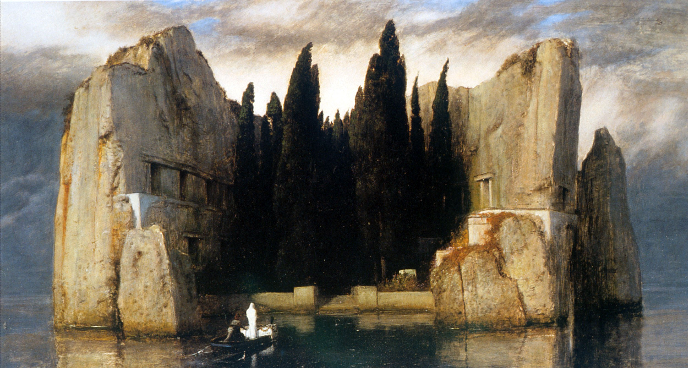
\includegraphics[width=0.2\textwidth]{imagenes/island.png} &
   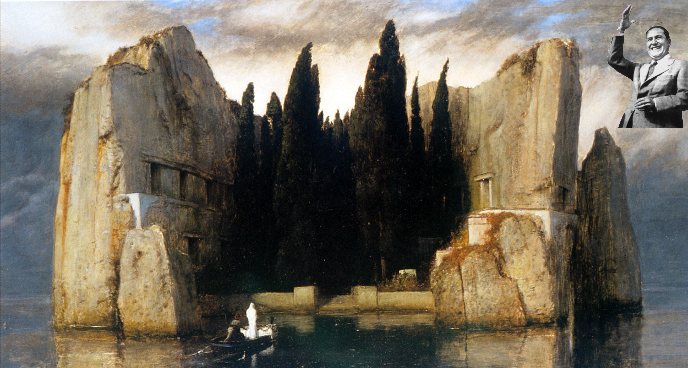
\includegraphics[width=0.2\textwidth]{imagenes/island-blit.png} &
   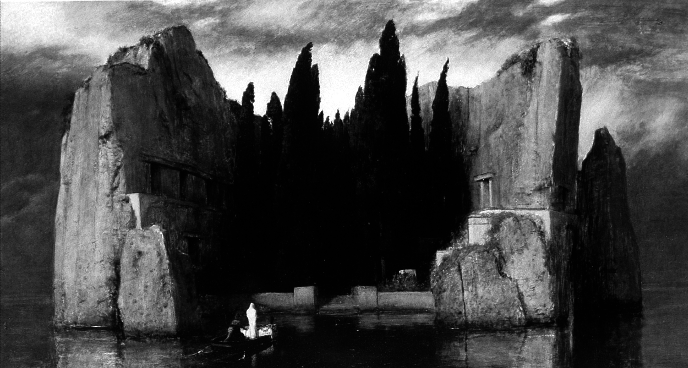
\includegraphics[width=0.2\textwidth]{imagenes/island-monocromatizar.png} \\
   Imagen original & Blit & Monocromatizar \\
   \\
   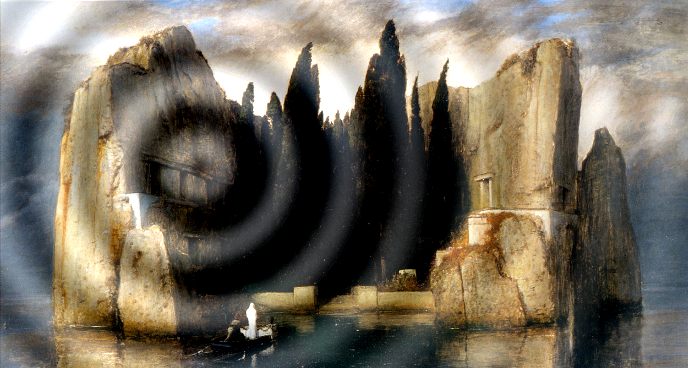
\includegraphics[width=0.2\textwidth]{imagenes/island-ondas.png} &
   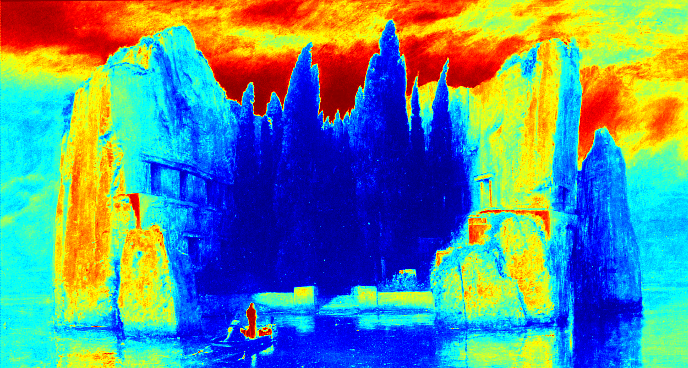
\includegraphics[width=0.2\textwidth]{imagenes/island-temperature.png} &
   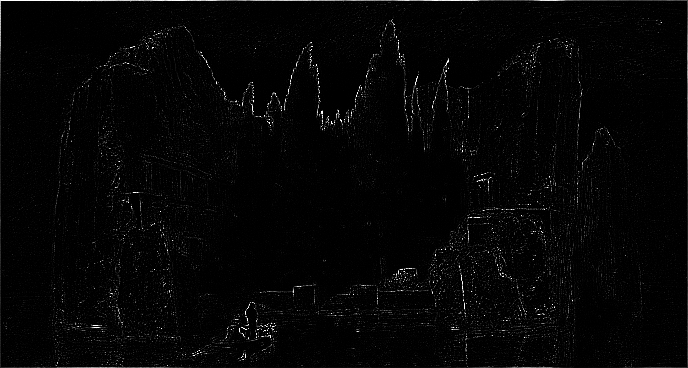
\includegraphics[width=0.2\textwidth]{imagenes/island-edge.png} \\
   Ondas & Temperature & Edge \\
 \end{tabular}
\end{center}

\subsection{Preliminares}

Consideramos a una imagen como una matriz de píxeles. Cada píxel está determinado por cuatro componentes: los colores azul (\Blue), verde (\Green) y rojo (\Red), y la transparencia (\Alpha). En nuestro caso particular cada una de estas componentes tendrá 8 bits (1 byte) de profundidad, es decir que estarán representadas por números enteros en el rango $[0,256)$.

% La cátedra provee una librería de funciones para cargar a memoria imágenes en formato BMP, de manera tal que su tarea se reduce a escribir funciones que trabajan con matrices de píxeles. (Detalles en sección~\ref{sec:

% Para la descripción de los filtros asumiremos una imagen de entrada $M$ de tamaño $m$ filas y $n$ columnas.

Dada una imagen $I$, notaremos $\mathsf{I}_{i,j}^k$ al valor de la componente $k \in \{ \Red, \Green, \Blue, \Alpha \}$ del píxel en la fila $i$ y la columna $j$ de la imagen.
La fila 0 corresponde a la fila de más abajo de la imagen.
La columna 0 a la de más a la izquierda.

Llamaremos $\mathsf{O}$ a la imagen de salida generada por cada filtro. Por ejemplo, el filtro identidad estaría caracterizado por la fórmula
\[ \forall k \in \{\Red,\Green,\Blue,\Alpha\} \quad \mathsf{O}_{i,j}^k = \mathsf{I}_{i,j}^k. \]

\subsection{Blit}

Esta operaci\'on recibe m\'as par\'ametros que las dem\'as; adem\'as de tener las im\'agenes fuente y destino (de tama\~no w x h), 
se recibe una imagen adicional \textbf{blit} tambi\'en con su respectivo tama\~no (bw x bh), que se utilizar\'a a modo de m\'ascara.
Se cumple que $bw \leq w \wedge bh \leq h$.\\

La aplicaci\'on de este filtro consiste en generar una nueva imagen combinando la original con el \textbf{blit}.
Un color de la imagen \textbf{blit} es considerado como transparente,
para que en la combinaci\'on algunos pixeles del \textbf{blit} queden por encima de la imagen original y otros no se vean.

Para este trabajo pr\'actico, la imagen \textbf{blit} ser\'a una imagen de Per\'on.
Decimos que una im\'agen ha sido ``Peronizada'' cuando en su extremo superior derecho podemos ver a Per\'on agitando su brazo.
% La aplicaci\'on de este filtro consiste en generar una nueva imagen combinando la original con la de Per\'on (blit) para as\'i 
% obtener una versi\'on ``Peronizada'' de la im\'agen fuente.

\vskip 8pt
Para cada p\'ixel $p$ en la imagen de Per\'on (blit):\\
$dst(p) = \begin{cases}
    src(p) & \mathrm{si \;} blit(p) \mathrm{\; es \; de \; color \; magenta, \; es \; decir \; sus \; colores \; son \;} (255, 0, 255)\\
    blit(p) & \mathrm{si \; no}
\end{cases}$ \\

Es decir que si el p\'ixel en la imagen de Per\'on es magenta, entonces el nuevo p\'ixel tendr\'a los colores del p\'ixel correspondiente 
en la imagen original; y si no los colores del p\'ixel en la imagen de Per\'on. \\

Las columnas y filas que no se puedan procesar de esta manera, es decir, 
las primeras $h - bh$ filas; y de las filas restantes, las primeras $w - bw$ columnas; 
quedar\'an igual que como estaban originalmente. \\

Nota: como debe valer la restricci\'on $bw \leq w \wedge bh \leq h$, esta operaci\'on 
no podr\'a ser aplicada a im\'agenes cuyo tama\~no sea menor a 89 p\'ixeles de ancho 
x 128 de alto.

%M\'as informaci\'on: http://en.wikipedia.org/wiki/Bit_blit

\subsubsection*{Implementación y uso}
\noindent Funciones: \code{blit_c}, \code{blit_asm}

\noindent Parámetros:
\begin{enumerate}[-]
\item \code{unsigned char *blit}: Imagen que se va a blitear
\item \code{int bh}: Alto de la imagen que se va a blitear
\item \code{int bw}: Ancho de la imagen que se va a blitear
\item \code{int b_row_size}: Bytes por fila de la imagen que se va a blitear
\end{enumerate}


% -----------------------------------------------------------------
% -----------------------------------------------------------------

\subsection{Monocromatizar norma $\inf$ } %(normas $1$ e $\inf$)}

Para convertir una imagen a escala de grises debemos contar con una funci'on 
que sea cap'az de monocromatizar una imagen a color. La funci'on m'as sencilla 
para hacer esto es:

\begin{center}
  $f(p) = \sqrt[\epsilon]{\alpha R^\epsilon + \beta G^\epsilon + 
    \gamma B^\epsilon}$
\end{center}

La funci'on $f$ se aplica a cada p'ixel $p$ de la imagen; $R$, $G$, $B$ son 
sus componentes de color, $\alpha$, $\beta$ y $\gamma$ son coeficientes entre 
$0$ y $1$, y $\epsilon$ es un exponente entre $1$ e $\infty$.\\

En nuestro caso se implementar'a la funci'on de conversi'on a escala de grises 
para un casos extremo, donde $\epsilon$ en la funci'on vale  
$\epsilon = \infty$. Adem'as, se fijar'an los par'ametros restantes en 
$\alpha = 1/4$, $\beta = 1/2$ y $\gamma = 1/4$. Luego, tenemos la siguiente
funcion para monocromatizar:

%para los casos extremos, donde $\epsilon$ en la funci'on vale $\epsilon = 1$ o 
%$\epsilon = \infty$. Adem'as, se fijar'an los par'ametros restantes en 
%$\alpha = 1/4$, $\beta = 1/2$ y $\gamma = 1/4$. Luego, tenemos dos posibles
%funciones para monocromatizar:

%\begin{center}
%  $I_{out\_uno}(p) = \frac{(R + 2G + B)}{4} (\epsilon = 1)$
%\end{center}

\begin{center}
  $I_{out\_infinito}(p) = max(R, G, B) (\epsilon = \infty)$
\end{center}


\subsubsection*{Implementación y uso}
\noindent Funciones: \\
\code{monocromatizar_inf_c}, \code{monocromatizar_inf_asm},
 
\noindent Parámetros: ninguno



% -----------------------------------------------------------------
% -----------------------------------------------------------------

\subsection{Efecto Ondas}

Deber'an implementar en \textbf{SSE} la funci'on ``ondas''. Esta combina la 
imagen original con una imagen de ondas, dando tonos m'as oscuros y m'as claros 
en forma de onda. Estas se generan desde el centro de la imagen hacia 
sus bordes de manera conc'entrica.\\

Para simplificar la tarea de programaci'on se proporciona una implementaci'on 
en C de este efecto en el archivo ``ondas\_c.c''.\\

El procedimiento a realizar es el siguiente:

\begin{algorithm}[H]
  \begin{algorithmic}[1]
    \FORALL{pixel ubicado en la posici'on $\mathbf{(x, y)}$}
      \STATE $d_x \gets x - x_0$

      \STATE

      \STATE $d_y \gets y - y_0$

      \STATE

      \STATE $d_{xy} \gets \sqrt{d_{x}^2+d_{y}^2}$

      \STATE

      \STATE $r \gets \frac{(d_{xy} - RADIUS)}{WAVELENGTH}$

      \STATE

      \STATE $a \gets \frac{1}{1 + (\frac{r}{TRAINWIDTH})^2 }$

      \STATE

      \STATE $t \gets ( r-floor(r) ) \cdot 2 \cdot \pi - \pi$

      \STATE

      \STATE $prof \gets a \cdot (t - \frac{t^3}{6}+\frac{t^5}{120}-\frac{t^7}{5040})$

      \STATE

      \STATE $pixel = prof \cdot 64 + I_{src}(x, y)$    

      \STATE

      \STATE $I_{dst}(x, y) = saturar(pixel)$
    \ENDFOR
  \end{algorithmic}
  \caption{$ondas (I_{src}, I_{dst}, x_0, y_0)$}
  \label{alg:ondas}
\end{algorithm}

donde:

\begin{itemize}
  \item $x_0$ e $y_0$ representan la posici'on donde est'a centrada la onda,
  \item $RADIUS$, $WAVELENGTH$ y $TRAINWIDTH$ son constantes que definen la 
  forma de la onda y
  \item $saturar(x)$ es una funci'on que retorna $0$ si $x$ es menor $0$, $255$
  si es mayor a $255$ y $x$ en cualquier otro caso.
\end{itemize}

\subsubsection*{Implementación y uso}

\noindent Funciones: \code{ondas_c}, \code{ondas_asm},

\noindent Parámetros: ninguno

\noindent Ejemplo de uso: \code{ondas -i c lena.bmp}




% -----------------------------------------------------------------
% -----------------------------------------------------------------

\subsection{Edge}

Puede definirse como un borde a los p\'ixeles donde la intensidad de la imagen cambia de forma abrupta. 
Si se considera una funci\'on de intensidad de la imagen, entonces lo que se busca son saltos en dicha funci\'on.
La idea b\'asica detr\'as de cualquier detector de bordes es el c\'alculo de un operador local de derivaci\'on. \\
 

Vamos a usar en este caso el operador de Laplace, cuya matriz es

$$ M = \left(
\begin{matrix}
    0.5 & 1 & 0.5 \\
    1 & -6 & 1 \\
    0.5 & 1 & 0.5
\end{matrix}
\right)$$


Para obtener los bordes, se posiciona el centro de la matr\'iz de 
Laplace en cada posici\'on $(x, y)$ y se realiza la siguiente operaci\'on

$$dst(x, y) = \sum_{k = 0}^2 \sum_{l = 0}^2 src(x + k - 1, y + l - 1) * M(k, l)$$

Es decir $dst(x, y) = $
\begin{center}
    $\begin{matrix}
        src(x - 1, y - 1) * M_{00} & + & src(x - 1, y) * M_{01} & + & src(x - 1, y + 1) * M_{02} & +\\
        src(x, y - 1) * M_{10} & + & src(x, y1) * M_{11} & + & src(x, y + 1) * M_{12} & +\\ 
        src(x + 1, y - 1) * M_{20} & + & src(x + 1, y) * M_{21} & + & src(x + 1, y + 1) * M_{22} &
    \end{matrix}$
\end{center}

Este filtro opera sobre imágenes en escala de grises (1 componente de color por píxel).
En los bordes que no se pueden procesar según la fórmula anterior (por estar a los costados de la
imagen), aplica la fórmula $dst(x, y) = src(x,y)$.

\subsubsection*{Implementación y uso}

\noindent Funciones: \code{edge_c}, \code{edge_asm}

\noindent Parámetros: ninguno




% -----------------------------------------------------------------
% -----------------------------------------------------------------

\subsection{Temperatura}

    El filtro temperatura toma una imagen fuente y genera un
    efecto que simula un mapa de calor. El filtro toma
    los tres componentes del cada pixel, los suma y divide por 3, y califica a eso
    como la temperatura $t$.

    \begin{center}
    $\mathsf{t}_{(i,j)} = \lfloor(\mathsf{src}.r_{(i,j)} + \mathsf{src}.g_{(i,j)} + \mathsf{src}.b_{(i,j)}) / 3\rfloor$
	\end{center}
    
    En función de la temperatura, se determina el color en la imagen destino. 
    Para evitar diferencias con los resultados la cátedra, la 
    temperatura debe truncarse y guardarse en una variable de tipo entero.

    \begin{center}
	\begin{displaymath}
	\mathsf{dst}_{(i,j)}<r,g,b> = \left\{
	\begin{array}{l l}
				<0,0, 128 + t \cdot 4> & \text{si }t < 32\\
				<0, (t - 32) \cdot 4, 255> & \text{si }32 \le t < 96\\
				<(t-96) \cdot 4, 255, 255 - (t-96) \cdot 4> & \text{si }96 \le t < 160\\
				<255, 255 - (t - 160) \cdot 4, 0> & \text{si }160 \le t < 224\\
				<255 - (t - 224) \cdot 4, 0 , 0> & \text{si no} \\
	\end{array}
	\right.
	\end{displaymath}
	\end{center}
	
    \newpage




\subsubsection*{Implementación y uso}

\noindent Funciones: \code{temperature_c}, \code{temperature_asm},

\noindent Parámetros: ninguno

\noindent Ejemplo de uso: \code{temperature -i c lena.bmp}


% -----------------------------------------------------------------
% -----------------------------------------------------------------



% ------------------------------------------------------------------
% ------------------------------------------------------------------

%\newpage
\section{Implementación}

Para facilitar el desarrollo del trabajo práctico se cuenta con un
\emph{framework} que provee todo lo necesario para poder leer y
escribir imágenes, así como también compilar y probar las funciones
que vayan a implementar.

\subsection{Archivos y uso}

\vspace*{0.3cm}
Dentro de los archivos presentados deben completar el código de las funciones
pedidas. Puntualmente encontrarán el programa principal (de línea de
comandos), denominado \textbf{tp2}, que se ocupa de parsear las opciones
ingresadas por el usuario y ejecutar el filtro seleccionado sobre la imagen
ingresada.

\vspace*{0.3cm}
\noindent Los archivos entregados están organizados en las siguientes carpetas:

\begin{itemize}
    \itemsep0em
    \item
        \code{documentos}: Contiene este enunciado y un \emph{template}
        de informe en \LaTeX.

	\item
		\code{codigo}: Contiene el código fuente, junto con el framework
		de ejecución y testeo.
		Contiene los fuentes del programa principal,
    		junto con el \textbf{Makefile} que permite compilarlo.
		Además contiene los siguientes subdirectorios:
		\begin{itemize}
		\item
			\code{build}: Contiene los archivos objeto y ejecutables
			del TP.

		\item
			\code{filtros}: Contiene las implementaciones de los filtros

		\item
			\code{helper}: Contiene los fuentes de la biblioteca BMP y
			de la herramienta de comparación de imágenes.

		\item
			\code{img}: Algunas imágenes de prueba.

    		\item
			\code{test}: Contiene scripts para realizar tests sobre los
	        filtros y uso de la memoria.
	\end{itemize}
\end{itemize}

\subsubsection*{Compilación}

Ejecutar \texttt{make} desde la carpeta \texttt{codigo}.
Recordar que cada directorio tiene su propio \code{Makefile},
por lo que si se desea cambiar las opciones de compilación
debe buscarse el \code{Makefile} correspondiente.

\subsubsection*{Uso}
% -----------------------------------------------------------------------------

\vspace*{0.2cm}
\noindent El uso del programa principal es el siguiente:
\vspace*{-0.2cm}
\begin{itemize}
    \item [\code{\$}]
        \code{./tp2 $<$opciones$>$ $<$nombre\_filtro$>$
              $<$nombre\_archivo\_entrada$>$ [parámetros...]}
\end{itemize}


Los filtros que se pueden aplicar y sus parámetros son
los especificados en la sección filtros, apartado
``Implementación y uso``


Las opciones que acepta el programa son las siguientes:
\begin{itemize}
  \itemsep0em
  \item \code{-h, --help} \\
  \indent Imprime la ayuda

  \item \code{-i, --implementacion NOMBRE\_MODO} \\
  \indent Implementación sobre la que se ejecutará el proceso
    seleccionado. Los implementaciones disponibles son: c, asm

  \item \code{-t, --tiempo CANT\_ITERACIONES} \\
  \indent Mide el tiempo que tarda en ejecutar el filtro sobre la
    imagen de entrada una cantidad de veces igual a CANT\_ITERACIONES

%  \item \code{-f, --frames} \\
%  \indent Genera frames independientes
%    en vez de armar un archivo de video. Es utilizado para testing. Sólo para archivos de video.

  \item \code{-o, --output DIRECTORIO} \\
  \indent Genera el resultado en DIRECTORIO.
    De no incluirse, el resultado se guarda en el mismo directorio
    que el archivo fuente

  \item \code{-v, --verbose} \\
  \indent Imprime información adicional

%  \item \code{-w, --video} \\
%  \indent Interpreta el archivo de entrada como video.
%    En caso de no estar, se interpreta la entrada como una imagen.

\end{itemize}

\vspace*{0.3cm}
\noindent Por ejemplo:
\vspace*{-0.2cm}
\begin{itemize}
    \item [\code{\$}]
        \code{./tp2 -v colorizar -i asm island.bmp 0.4}
\end{itemize}

\noindent Aplica el filtro de \textbf{colorizar} al archivo island.bmp
utilizando la implementación en lenguaje asm del filtro, pasándole como parámetro 0.4 como valor de alpha.

\subsection{Código de los filtros}

Para implementar los filtros descriptos anteriormente, tanto en C como
en ASM se deberán implementar las funciones especificadas en la sección
\ref{filtros}.
Las imágenes se almacenan en memoria en color, en el orden
B (blue), G (green), R (red), A (alpha).

% -----------------------------------------------------------------------------
Los parámetros genéricos de las funciones son:
\begin{itemize}
  \itemsep0em
  \item[-]
      \code{src}\rmfamily: Es el puntero al inicio de la matriz de
      elementos de 32 bits sin signo (el primer byte corresponde al canal azul
      de la imagen (B), el segundo el verde (G), el tercero el rojo (R)), y el
      cuarto el alpha (A) que
      representa a la imagen de entrada. Es decir, como la imagen está en
      color, cada píxel está compuesto por 4 bytes.

   \item[-]
      \code{dst}\rmfamily: Es el puntero al inicio de la matriz de
      elementos de 32 bits sin signo que representa a la imagen de salida.

   \item[-]
      \code{filas}\rmfamily: Representa el alto en píxeles de la imagen, es
      decir, la cantidad de filas de las matrices de entrada y salida.

   \item[-]
      \code{cols}\rmfamily: Representa el ancho en píxeles de la imagen, es
      decir, la cantidad de columnas de las matrices de entrada y salida.

   \item[-]
      \code{src\_row\_size}\rmfamily: Representa el ancho en bytes de cada fila
      de la imagen incluyendo el padding en caso de que hubiere. Es decir, la cantidad de bytes que hay que avanzar para moverse a la misma columna de fila siguiente/anterior.
\end{itemize}

% --------------------------------------------------------------------
% --------------------------------------------------------------------

%\newpage
\subsubsection*{Consideraciones}

Las funciones a implementar en lenguaje ensamblador deben utilizar el set de
instrucciones \textbf{SSE}, a fin de optimizar la performance de las mismas.
Tener en cuenta lo siguiente:

\begin{itemize}
  \itemsep0em
  \item El ancho de las imágenes es siempre mayor a 16 píxeles y múltiplo de 4 píxeles.

  \item No se debe perder precisión en ninguno de los cálculos, a menos que se indique lo contrario.

  \item La implementación de cada filtro deberá estar optimizada para el
    filtro que se está implementando. No se puede hacer una función que
    aplique un filtro genérico y después usarla para implementar los que se
    piden.

  \item Para el caso de las funciones implementadas en lenguaje ensamblador,
    deberán trabajar con \textbf{al menos 2 píxeles simultámeamente}.

    De no ser posible esto para algún filtro, deberá justificarse
    debidamente en el informe.

  \item El procesamiento de los píxeles se deberá hacer
    \textbf{exclusivamente} con instrucciones \textbf{SSE}.
    No está permitido procesarlos con registros de propósito general,
    salvo para tratatimiento de casos borde. En tal caso se deberá
    justificarse debidamente y hacer un análisis del costo computacional.

  \item El TP se tiene que poder ejecutar en las máquinas del laboratorio.
\end{itemize}



\subsection{Formato BMP}

El formato BMP es uno de los formatos de imágenes mas simples: tiene un encabezado y un mapa de bits que representa la información de los pixeles.
En este trabajo práctico se utilizará una biblioteca provista por la cátedra para operar con archivos en ese formato.
Si bien esta biblioteca no permite operar con archivos con paleta, es posible leer tres tipos de formatos, tanto con o sin transparencia.
Ambos formatos corresponden a los tipos de encabezado: BITMAPINFOHEADER (40 bytes), BITMAPV3INFOHEADER (56 bytes) y BITMAPV5HEADER (124 bytes).
\smallskip

El código fuente de la biblioteca está disponible como parte del material, deben seguirlo y entenderlo.
Las funciones que deben implementar reciben como entrada un puntero a la imagen. Este puntero corresponde al mapa de bits almacenado en el archivo.
El mismo está almacenado de forma particular: \textbf{las líneas de la imagen se encuentran almacenadas de forma invertida}.
Es decir, en la primera fila de la matriz se encuentra la última línea de la imagen, en la segunda fila se encuentra la anteúltima y así sucesivamente.
Dentro de cada línea los pixeles se almacenan de izquierda a derecha, y cada pixel \textbf{en memoria se guarda en el siguiente orden: B, G, R, A}.



% -----------------------------------------------------------------
% -----------------------------------------------------------------

\subsection{Herramientas y tests}

En el código provisto, podrán encontrar varias herramientas
que permiten verificar si los filtros funcionan correctamente.

\subsubsection*{Diff}
La herramienta \code{diff} permite comparar dos imágenes.
El código de la misma se encuentra en \texttt{helper}, y se
compila junto con el resto del trabajo práctico.
El ejecutable, una vez compilado, se almacenará en
\texttt{build/bmpdiff}.
La aplicación se utiliza desde linea de comandos de la forma:

\begin{codesnippet}
./build/bmpdiff $<$opciones$>$ $<$archivo_1$>$ $<$archivo_2$>$ $<$epsilon$>$
\end{codesnippet}


Esto compara los dos archivos según las componentes de cada pixel, siendo epsilon la diferencia máxima permitida entre pixeles correspondientes de las dos imágenes.
Tiene dos opciones: listar las diferencias o generar imágenes blanco y negro por cada componente, donde blanco es marca que hay diferencia y negro que no.

\bigskip
Las opciones soportadas por el programa son:

\begin{tabular}{l|l}
  \verb|-i|, \verb|--image|    &  Genera imágenes de diferencias por cada componente.\\
  \verb|-v|, \verb|--verbose|  &  Lista las diferencias de cada componente y su posición en la imagen.\\
  \verb|-a|, \verb|--value|    &  Genera las imágenes mostrando el valor de la diferencia.\\
  \verb|-s|, \verb|--summary|  &  Muestra un resumen de diferencias.\\
\end{tabular}

\subsubsection*{Tests}
Para verificar el correcto funcionamiento de los filtros,
además del comparador de imágenes, se provee un binario
con la solución de la cátedra y varios scripts de test.
El binario de la cátedra se encuentra en la carpeta {\code{codigo/build}}.
El comparador de imágenes se ubica en la carpeta {\code{codigo/helper}}, y debe
compilarse antes de correr los scripts (correr {\code{make}} en la carpeta {\code{codigo/helper}}).

Los scripts de test toman como entrada las corridas especificadas en {\code{corridas.txt}}.
Para cada imagen de test, se ejecutan todas las corridas ahí indicadas.
Para verificar que la implementación funciona correctamente con imágenes de distinto
tamaño,{ \code{generar\_imagenes.sh}} genera variaciones de las imágenes fuente
(que se encuentran en {\code{codigo/tests/data}}), y las deposita en {\code{imagenes\_a\_testear}}.
Para que este script funcione correctamente se requiere la utilidad {\code{convert}} que se encuentra
en la biblioteca {\code{imagemagick}}.\footnote{Para instalar \code{sudo apt-get install imagemagick}}.

El archivo {\code{test\_dif\_cat.sh}} verifica que los resultados de la catedra den igual que la implementación de C.
{\code{test\_dif\_c\_asm.sh}} verifica que los resultados de las versiones de C y Assembler sean iguales.
{\code{test\_mem.sh}} chequea que no haya problemas en el uso de la memoria.
Finalmente, {\code{test\_all.sh}} corre todos los checks anteriores uno después del otro.

\subsection{Mediciones de rendimiento}

La forma de medir el rendimiento de nuestras implementaciones se realizará por medio de la toma de tiempos de ejecución.
Como los tiempos de ejecución son muy pequeños, se utilizará uno de los contadores de performance que posee el procesador.

La instrucción de assembler \texttt{rdtsc} permite obtener el valor del Time Stamp Counter (TSC) del procesador.
Este registro se incrementa en uno con cada ciclo del procesador.
Obteniendo la diferencia entre los contadores antes y después de la llamada a la función, podemos obtener la cantidad de ciclos de esa ejecución.
Esta cantidad de ciclos no es siempre igual entre invocaciones de la función, ya que este registro es global del procesador y se ve afectado por una serie de factores.

Existen principalmente distintas problemáticas a solucionar:

\begin{enumerate}
 \item La ejecución puede ser interrumpida por el \emph{scheduler} para realizar un cambio de contexto, esto implicará contar muchos más ciclos (\emph{outliers}) que si nuestra función se ejecutara sin interrupciones.
 \item Los procesadores modernos varían su frecuencia de reloj, por lo que la forma de medir ciclos cambiará dependiendo del estado del procesador.
 \item El comienzo y fin de la medición deben realizarse con la suficiente
 exactitud como para que se mida solamente la ejecución de los filtros, sin
 ser afectada por ruidos como la carga o el guardado de las imágenes.
\end{enumerate}

Para medir tiempos deberán idear e implementar una metodología que les permita evitar estos tres problemas.
En el archivo \texttt{tp2.c} se provee código para realizar una
medición de tiempo básica. El mismo podrá ser modificado para
mejorar y automatizar las mediciones.
Se recomienda utilizar un framework de medición automatizado
como \code{metrika}\footnote{pip3 install --user metrika |
\url{https://github.com/dc-uba/metrika}}
para evitar errores de medición sistemáticos, es decir, aquellos
causados por una incorrecta ejecucción de las mediciones.



% ---------------------------------------------------------------------
% ---------------------------------------------------------------------


\section{Ejercicios}

Se deberá implementar el código de los filtros, realizar
un análisis de su performance y presentar un informe de los
resultados.

\subsection{Implementación}

Deberán implementar (al menos) una versión de cada filtro en C y otra en lenguaje ensamblador, utilizando instrucciones SSE.
La implementación inicial de los filtros que sólo realicen cálculos
con números enteros no deberá perder precisión. Es posible que se
desee realizar optimizaciones al costo de perder algo de precisión.
Esto será aceptable siempre y cuando se analice también la calidad
de la imagen resultante en la versión optimizada contra la no
optimizada.

\subsection{Análisis}

Las siguientes preguntas deben ser usadas como guía.
La evaluación del trabajo práctico no sólo consiste en responder
las preguntas, sino en desarrollar y responder nuevas preguntas
sugeridas por ustedes mismos buscando entender y razonar sobre
el modelo de programación SIMD y la microarquitectura del procesador.


\begin{itemize}
\item ¿Cuál implementación es ``mejor''?
\item ¿Qué métricas se pueden utilizar para calificar las implementaciones y cuantificarlas?
\item ¿En qué casos? ¿De qué depende? ¿Depende del tamaño de la imagen? ¿Depende de la imagen en sí? ¿De los parámetros?
\item ¿Cómo se podrían mejorar las métricas de las implementaciones propuestas? ¿Cuáles no se pueden mejorar?
\item ¿Es una comparación justa? ¿De qué depende la velocidad del
código C? ¿Cómo puede optimizarse?
\item ¿Cuál es la cantidad de instrucciones ejecutadas por pixel en cada implementación? ¿Y de accesos a memoria? ¿Se condice empíricamente esta diferencia en la performance de los filtros?
\item ¿Hay diferencias en operar con enteros o punto flotante? ¿La imagen final tiene diferencias significativas?
\item ¿El overhead de llamados a funciones es significativo? ¿Se puede medir?
\item ¿Las limitaciones de performance son causadas por los accesos a memoria?, ¿o a la memoria cache?, ¿esta se podría acceder mejor?
\item ¿Y los saltos condicionales? ¿Afectan la performance? ¿Es posible evitarlos total o parcialmente?
\item ¿El patrón de acceso a la memoria es desalineado? ¿Hay forma de mejorarlo? ¿Es posible medir cuánto se pierde?
\end{itemize}


\subsection{Informe}

El informe debe incluir las siguientes secciones:

\begin{enumerate}
    \item
        \textbf{Carátula} Contiene

        \begin{itemize}
            \item número / nombre del grupo
            \item nombre y apellido de cada integrante
            \item número de libreta y mail de cada integrante
        \end{itemize}

    \item
        \textbf{Introducción}
        Describe lo realizado en el trabajo práctico.

    \item
        \textbf{Desarrollo}\\
        Describe cada una de las funciones que implementaron.
	    Para la descripción de cada función deberán decir cómo
        opera una iteración del ciclo de la función.
        Es decir, cómo mueven los datos a los registros, cómo los
        reordenan para procesarlos, las operaciones que se aplican
        a los datos, etc.
        Además se agregará un detalle más profundo de las secciones
        de código que consideren más importantes.
        Para esto pueden utilizar pseudocódigo, diagramas (mostrando
        gráficamente el contenido de los registros \texttt{XMM}) o
        cualquier otro recurso que le sea útil para describir la
        adaptación del algoritmo al procesamiento simultáneo SIMD.
        No se deberá incluir el código assembler de las funciones
        (aunque se pueden incluir extractos en donde haga falta).

	\item
		\textbf{Resultados}\\
		Deberán \textbf{analizar} y \textbf{comparar} las
		implementaciones de las funciones en su versión \textbf{C}
		y \textbf{assembler} y mostrar los resultados obtenidos a
		través de tablas y gráficos.
		Para esto deberán plantear experimentos que les permitan
		comprobar las diferencias de performance e hipotetizar
		sobre sus causas.

		Deberán además explicar detalladamente los resultados
		obtenidos y analizarlos.
		En el caso de encontrar anomalías o comportamientos no
		esperados deberán construir nuevos experimentos para
		entender qué es lo que sucede.


	    Utilizar como guía para la realización de experimentos
	    las preguntas de la sección anterior.
	    Al responder estas preguntas (y otras que vayan surgiendo),
	    se deberán analizar y comparar
        las implementaciones de cada funcion en su versión
        \texttt{C} y \texttt{ASM}, mostrando los resultados obtenidos
        a través de tablas y gráficos.
        También se deberá \emph{comentar} los resultados obtenidos.
	    %En el caso de que sucediera que la versión en C anduviese más
        %rápidamente que su versión ASM, \textbf{justificar
        %fuertemente} a qué se debe esto.

    \item
        \textbf{Conclusión}
        Reflexión final sobre los alcances del trabajo práctico,
        la programación vectorial a bajo nivel,
        problemáticas encontradas, y todo lo que consideren pertinente.
\end{enumerate}

%El informe no puede exceder las \textbf{20} páginas, sin contar la
%carátula.

\vspace*{0.3cm}
\textbf{Importante}: El informe se evalúa de manera independiente del
código.
Puede reprobarse el informe, y en tal caso deberá ser reentregado para
aprobar el trabajo práctico.


% --------------------------------------------------------------------
% --------------------------------------------------------------------

\section{Entrega y condiciones de aprobación}

El presente trabajo es de carácter \textbf{grupal}, siendo los grupos de
\textbf{3 personas}, pudiendo ser de 2 personas en casos excepcionales previa
consulta y confirmación del cuerpo docente. Se deberá entregar un archivo
comprimido con el mismo contenido que el dado para realizarlo, habiendo
modificado sólo los archivos que tienen como nombre las funciones a
implementar. \textbf{No} debe incluírse ningún tipo de archivo binario extra
como código objeto o ejecutables.\\

%\textbf{Es codición necesaria para la aprobación de este trabajo que pasen correctamente
%todos los tests de la catedra.}

La fecha de entrega última de este trabajo es \textbf{Jueves 10 de Mayo}. Deberá ser entregado a través de un repositorio GIT almacenado en \url{https://git.exactas.uba.ar} respetando el protocolo enviado por mail y publicado en la página web de la materia.  La fecha límite para la \textbf{reentrega} es el día \textbf{Jueves 31 de Mayo.}\\

Ante cualquier problema con la entrega, comunicarse por
mail a la \textbf{lista de docentes}.\\

\end{document}

%\input{1-intro}

\section{Conclusiones y trabajo futuro}


\end{document}

